\documentclass[12pt,a4paper]{article}

% ── Paquetes ──────────────────────────────────────────────────────────────────
\usepackage[utf8]{inputenc}
\usepackage[T1]{fontenc}
\usepackage[spanish,es-nodecimaldot]{babel}

\usepackage{geometry}
\usepackage{amsmath,amssymb,amsthm}
\usepackage{booktabs}
\usepackage{array}
\usepackage{graphicx}
\usepackage{float}
\usepackage{caption}
\usepackage{subcaption}
\usepackage{hyperref}
\usepackage{parskip}
\usepackage{enumitem}
\usepackage{xcolor}
\usepackage{fancyhdr}
\usepackage{titlesec}
\usepackage{siunitx}

\geometry{
  top=2.5cm, bottom=2.5cm,
  left=3cm,  right=2.5cm
}

% ── Cabecera / pie ────────────────────────────────────────────────────────────
\pagestyle{fancy}
\fancyhf{}
\fancyhead[L]{\small Econometría -- UPTC}
\fancyhead[R]{\small Emanuel Quintana Silva}
\fancyfoot[C]{\thepage}
\renewcommand{\headrulewidth}{0.4pt}

% ── Formato de secciones ──────────────────────────────────────────────────────
\titleformat{\section}[block]{\normalfont\large\bfseries}{(\Alph{section})}{0.6em}{}
\titleformat{\subsection}[runin]{\normalfont\bfseries}{}{0pt}{}[.\enspace]

% ── Comandos propios ──────────────────────────────────────────────────────────
\newcommand{\Hcero}{H_0}
\newcommand{\Huno}{H_1}
\newcommand{\uhat}{\hat{u}}
\newcommand{\betahat}{\hat{\beta}}

% ── Hiperenlaces neutros ──────────────────────────────────────────────────────
\hypersetup{colorlinks=true,linkcolor=black,urlcolor=black,citecolor=black}

% ─────────────────────────────────────────────────────────────────────────────
\begin{document}

% ── Portada ───────────────────────────────────────────────────────────────────
\begin{titlepage}
  \centering
  \vspace*{2cm}
  {\Large \textsc{Universidad Pedagógica y Tecnológica de Colombia}\\[0.3cm]
   \large Escuela de Ciencias Economicas y Administrativas}\par
  \vspace{2cm}
  \rule{\linewidth}{0.6pt}\\[0.4cm]
  {\LARGE \bfseries Taller de Econometría}\\[0.3cm]
  {\large Autocorrelación: Diagnóstico y Corrección}\\[0.1cm]
  \rule{\linewidth}{0.6pt}
  \vspace{1.5cm}

  \begin{tabular}{rl}
    \textbf{Estudiante:} & Emanuel Quintana Silva \\[0.4em]
    \textbf{Curso:}      & Econometría \\[0.4em]
    \textbf{Datos:}      & Precio interno del cobre, EE.UU., 1951--1980 \\[0.4em]
    \textbf{Fuente:}     & Gujarati \& Porter (2010), Tabla 12.7 \\[0.4em]
    \textbf{Fecha:}      & 14 de abril de 2026
  \end{tabular}

  \vspace{2cm}
  \textit{Modelo log-log estimado por Mínimos Cuadrados Ordinarios:}\\[0.6em]
  \[
    \ln C_t = \beta_1 + \beta_2\ln I_t + \beta_3\ln L_t + \beta_4\ln A_t + u_t
  \]

  \vfill
\end{titlepage}

% ── Tabla de contenidos ───────────────────────────────────────────────────────
\tableofcontents
\newpage

% =============================================================================
\section{Estimación OLS del modelo log-log e interpretación}
\label{sec:A}
% =============================================================================

\subsection{Definición de variables}

El modelo analiza los determinantes del precio interno del cobre en los
Estados Unidos durante el período 1951--1980 mediante una especificación
doble-logarítmica:

\begin{equation}
  \ln C_t = \beta_1 + \beta_2\ln I_t + \beta_3\ln L_t + \beta_4\ln A_t + u_t
  \label{eq:modelo}
\end{equation}

\noindent donde:
\begin{itemize}[leftmargin=2cm]
  \item $C_t$: precio promedio (doce meses) del cobre en EE.UU.\ (centavos/libra)
  \item $I_t$: índice promedio (doce meses) de la producción industrial
  \item $L_t$: precio promedio (doce meses) del cobre en la bolsa de metales
               de Londres (libras esterlinas)
  \item $A_t$: precio promedio (doce meses) del aluminio (centavos de dólar/libra)
\end{itemize}

\subsection{Resultados de la estimación}

La Tabla~\ref{tab:ols} presenta los resultados de la regresión por MCO
estimada con Stata.

\begin{table}[H]
  \centering
  \caption{Estimación MCO --- Modelo log-log (Variable dependiente: $\ln C_t$)}
  \label{tab:ols}
  \small
  \begin{tabular}{lrrrrrr}
    \toprule
    Variable & Coeficiente & Error est. & $t$ & $P>|t|$ & IC 95\% inf. & IC 95\% sup. \\
    \midrule
    $\ln I_t$    & 0.4671 & 0.1614 & 2.89 & 0.008 & 0.1354 & 0.7988 \\
    $\ln L_t$    & 0.2807 & 0.1151 & 2.44 & 0.022 & 0.0442 & 0.5173 \\
    $\ln A_t$    & 0.4389 & 0.1049 & 4.18 & 0.000 & 0.2233 & 0.6545 \\
    Constante    & $-1.5344$ & 0.2765 & $-5.55$ & 0.000 & $-2.1028$ & $-0.9660$ \\
    \midrule
    \multicolumn{7}{l}{$n=30$\quad $R^2=0{,}9345$\quad $\bar{R}^2=0{,}9269$\quad
      $F(3,26)=123{,}61$ ($p<0{,}0001$)\quad RCME $=0{,}1209$} \\
    \bottomrule
  \end{tabular}
\end{table}

\subsection{Ecuación estimada}

\begin{equation}
  \widehat{\ln C_t} = -1{,}5344 + 0{,}4671\ln I_t + 0{,}2807\ln L_t + 0{,}4389\ln A_t
  \label{eq:estimada}
\end{equation}

\subsection{Interpretación económica de los coeficientes}

En un modelo log-log cada coeficiente es directamente una \textbf{elasticidad}:

\begin{enumerate}
  \item \textbf{$\hat{\beta}_2 = 0{,}4671$ (elasticidad respecto a $I_t$):}
    Un aumento de 1\% en el índice de producción industrial eleva el precio
    interno del cobre en aproximadamente \textbf{0,47\%}, \textit{ceteris paribus}.
    Esto refleja el efecto demanda: mayor actividad industrial presiona al alza
    el precio del cobre. El coeficiente es positivo y estadísticamente
    significativo ($p=0{,}008$).

  \item \textbf{$\hat{\beta}_3 = 0{,}2807$ (elasticidad respecto a $L_t$):}
    Un incremento de 1\% en el precio del cobre en Londres se asocia con un
    aumento de \textbf{0,28\%} en el precio doméstico. Esto es coherente con
    la integración de los mercados internacionales del cobre; la relación no es
    uno a uno porque existen fricciones (aranceles, costos de transporte,
    diferencias de calidad). Significativo al 5\% ($p=0{,}022$).

  \item \textbf{$\hat{\beta}_4 = 0{,}4389$ (elasticidad respecto a $A_t$):}
    Un aumento de 1\% en el precio del aluminio eleva el precio del cobre en
    \textbf{0,44\%}. El aluminio es un sustituto industrial del cobre:
    cuando el aluminio se encarece, la demanda se desplaza hacia el cobre,
    elevando su precio. Es el coeficiente más preciso ($p<0{,}001$).

  \item \textbf{Constante $\hat{\beta}_1 = -1{,}5344$:}
    Logaritmo del factor de escala del modelo; no tiene interpretación
    económica directa, aunque su significancia confirma que el modelo no
    debería estimarse sin término independiente.
\end{enumerate}

\subsection{Bondad del ajuste}

El modelo explica el 93,45\% de la variación en $\ln C_t$ ($R^2=0{,}9345$),
y el ajustado ($\bar{R}^2=0{,}9269$) es prácticamente igual, lo que indica
que los tres regresores son conjuntamente relevantes. El estadístico $F$
($=123{,}61$, $p<0{,}0001$) rechaza la hipótesis nula de que todos los
coeficientes son simultáneamente cero.

% =============================================================================
\section{Residuos y diagnóstico visual de autocorrelación}
\label{sec:B}
% =============================================================================

\subsection{Obtención de residuos}

Los residuos MCO se definen como
\[
  \hat{u}_t = \ln C_t - \widehat{\ln C_t}, \qquad t=1951,\ldots,1980.
\]

\subsection{Gráficas de diagnóstico}

\begin{figure}[H]
  \centering
  \begin{subfigure}[t]{0.90\textwidth}
    \centering
    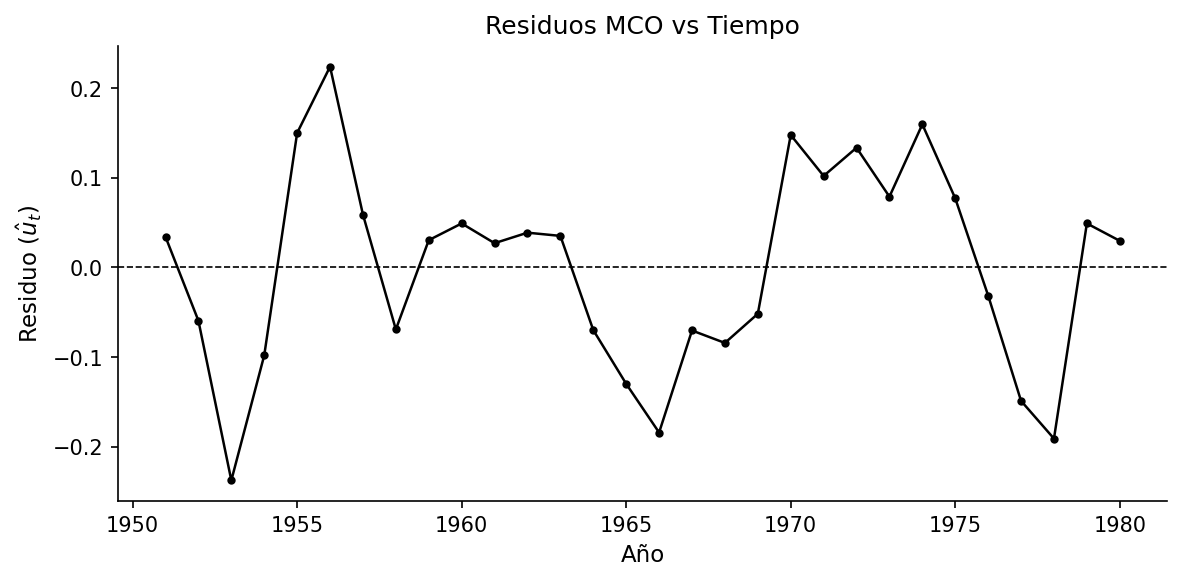
\includegraphics[width=\linewidth]{graf_residuos_tiempo.png}
    \caption{Residuos MCO a lo largo del tiempo (1951--1980).}
    \label{fig:res_tiempo}
  \end{subfigure}
  \vspace{0.8em}
  \begin{subfigure}[t]{0.55\textwidth}
    \centering
    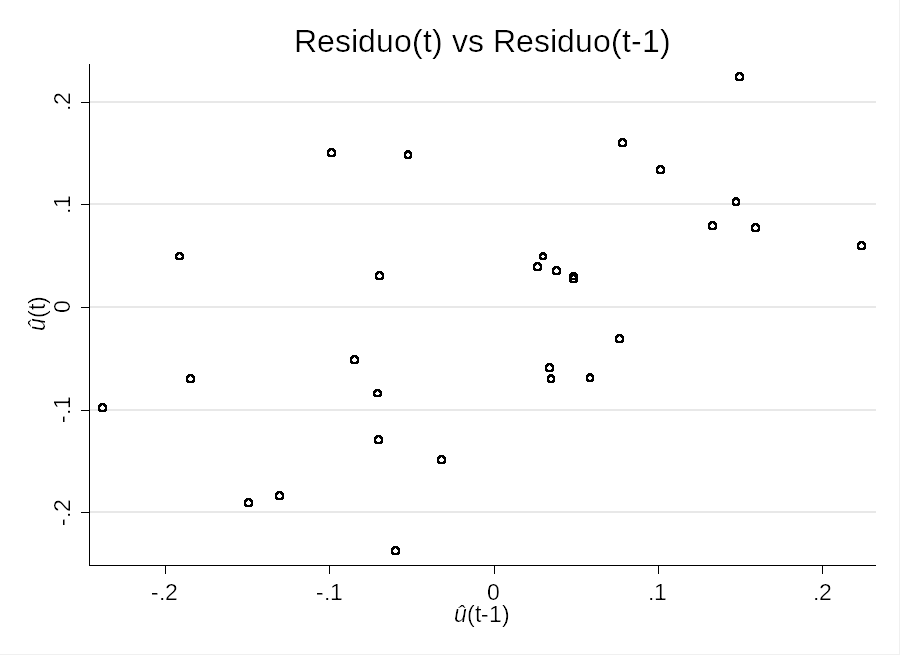
\includegraphics[width=\linewidth]{graf_residuos_lag.png}
    \caption{Diagrama de dispersión $\hat{u}_t$ vs.\ $\hat{u}_{t-1}$.}
    \label{fig:res_lag}
  \end{subfigure}
  \caption{Diagnóstico gráfico de autocorrelación en los residuos MCO.}
  \label{fig:residuos}
\end{figure}

\subsection{Interpretación}

\textbf{Figura~\ref{fig:res_tiempo} (residuos vs.\ tiempo):}
Los residuos no oscilan aleatoriamente alrededor de cero. Se observan
\emph{clusters} de residuos positivos (p.ej., 1956--1957 y 1973--1974) y
clusters de residuos negativos (1951--1955, 1958--1963), lo que es un patrón
característico de \textbf{autocorrelación positiva}: valores grandes van
seguidos de valores grandes del mismo signo.

\textbf{Figura~\ref{fig:res_lag} ($\hat{u}_t$ vs.\ $\hat{u}_{t-1}$):}
La nube de puntos se agrupa claramente en el primer y tercer cuadrante,
mostrando una relación positiva entre $\hat{u}_t$ y $\hat{u}_{t-1}$.
Esto es evidencia visual de autocorrelación de primer orden AR(1).

\textbf{Conclusión preliminar:} Las gráficas sugieren la presencia de
autocorrelación positiva en los errores, lo que viola el supuesto clásico
de errores no correlacionados. MCO sigue siendo insesgado pero ya no es
eficiente (BLUE falla), y los errores estándar están subestimados, lo que
infla los estadísticos $t$.

% =============================================================================
\section{Estadístico de Durbin-Watson}
\label{sec:C}
% =============================================================================

\subsection{Hipótesis y estadístico}

La prueba de Durbin-Watson contrasta:
\[
  \Hcero: \rho = 0 \quad\text{(no hay autocorrelación de primer orden)}
  \qquad\text{vs.}\qquad
  \Huno: \rho > 0 \quad\text{(autocorrelación positiva)}
\]

El estadístico se define como:
\begin{equation}
  d = \frac{\displaystyle\sum_{t=2}^{n}(\hat{u}_t - \hat{u}_{t-1})^2}
           {\displaystyle\sum_{t=1}^{n}\hat{u}_t^2}
  \approx 2(1-\hat{\rho})
  \label{eq:dw}
\end{equation}

\subsection{Resultado de Stata}

\[
  \boxed{d = 0{,}9428}
\]

\subsection{Región de decisión}

Con $n=30$ observaciones, $k'=3$ regresores y $\alpha=5\%$, los valores
críticos de la tabla Durbin-Watson son:

\[
  d_L = 1{,}21 \qquad d_U = 1{,}65
\]

\begin{center}
\begin{tabular}{ccccc}
  \toprule
  $0$ & $d_L=1{,}21$ & $d_U=1{,}65$ & $4-d_U=2{,}35$ & $4-d_L=2{,}79$ \\
  \midrule
  Autocorr.\ & Zona  & No rechaza & Zona  & Autocorr. \\
  positiva   & ind.  & $H_0$      & ind.  & negativa  \\
  \bottomrule
\end{tabular}
\end{center}

Como $d = 0{,}9428 < d_L = 1{,}21$, la estadística cae en la región de
\textbf{rechazo de $H_0$}: existe evidencia de \textbf{autocorrelación
positiva de primer orden}.

\subsection{Estimación de $\rho$}

A partir de la aproximación $d \approx 2(1-\hat\rho)$:
\[
  \hat\rho \approx 1 - \frac{d}{2} = 1 - \frac{0{,}9428}{2} \approx 0{,}529
\]

Esto indica una correlación serial moderada-alta y positiva entre errores
consecutivos.

\subsection{Limitaciones del estadístico DW}

\begin{itemize}
  \item Solo detecta autocorrelación de \emph{primer} orden.
  \item La zona de indecisión puede ser amplia para muestras pequeñas.
  \item No es válido cuando la regresión incluye variables dependientes
        rezagadas como regresores.
  \item Con modelos de series de tiempo largas pueden preferirse las
        pruebas de Breusch-Godfrey (ver sección~\ref{sec:E}).
\end{itemize}

% =============================================================================
\section{Prueba de Rachas (Wald-Wolfowitz)}
\label{sec:D}
% =============================================================================

\subsection{Fundamento}

La prueba de rachas (runs test) es una prueba no paramétrica que evalúa la
aleatoriedad de la secuencia de signos de los residuos, sin asumir ninguna
distribución específica para los errores.

Una \emph{racha} es una sucesión de observaciones del mismo signo; si los
residuos son verdaderamente aleatorios, el número de rachas $R$ se distribuye
aproximadamente de forma normal para muestras grandes.

\subsection{Hipótesis}

\[
  \Hcero: \text{los residuos son aleatorios (no hay autocorrelación)}
  \qquad\text{vs.}\qquad
  \Huno: \text{no son aleatorios (hay autocorrelación)}
\]

\subsection{Estadístico}

Sea $n_1$ el número de residuos positivos y $n_2$ el número de residuos
negativos. El estadístico es:

\[
  z = \frac{R - \bar{R}}{\sigma_R}, \qquad
  \bar{R} = \frac{2n_1 n_2}{n_1+n_2}+1, \qquad
  \sigma_R^2 = \frac{2n_1 n_2(2n_1 n_2-n_1-n_2)}{(n_1+n_2)^2(n_1+n_2-1)}
\]

\subsection{Resultado de Stata}

\begin{center}
\begin{tabular}{ll}
  \toprule
  Residuos $\leq 0$ & $n_2 = 13$ \\
  Residuos $> 0$    & $n_1 = 17$ \\
  Total             & $n = 30$   \\
  Número de rachas  & $R = 9$    \\
  \midrule
  Estadístico $z$   & $-2{,}55$ \\
  $p$-valor (bilateral) & $0{,}0108$ \\
  \bottomrule
\end{tabular}
\end{center}

El número esperado de rachas bajo aleatoriedad es:
\[
  \bar{R} = \frac{2(17)(13)}{30}+1 = \frac{442}{30}+1 \approx 15{,}73
\]

Solo se observaron 9 rachas, muy por debajo del valor esperado de
$\approx 15{,}7$.

\subsection{Decisión}

Con $|z|=2{,}55 > 1{,}96$ y $p=0{,}011<0{,}05$, se rechaza $H_0$ al nivel
del 5\%. Los residuos \textbf{no son aleatorios}.

\subsection{Comparación con Durbin-Watson (punto C)}

Ambas pruebas coinciden en su conclusión: los residuos exhiben
\textbf{autocorrelación positiva}. Sin embargo, la prueba de rachas aporta
información adicional:

\begin{itemize}
  \item \textbf{DW} asume normalidad de los errores y está diseñada
        específicamente para AR(1). Dio $d=0{,}9428<d_L$, evidenciando
        autocorrelación positiva.

  \item \textbf{Rachas} es no paramétrica: no exige ninguna distribución
        para $u_t$, y detecta cualquier patrón de no aleatoriedad
        (no solo AR(1)). Con $R=9 \ll \bar{R}\approx 15{,}7$ y $z=-2{,}55$,
        apunta a la misma dirección.

  \item La consistencia entre ambas pruebas refuerza la evidencia: la
        violación del supuesto de no autocorrelación parece robusta y
        no dependiente de los supuestos distribucionales.
\end{itemize}

% =============================================================================
\section{Prueba del Multiplicador de Lagrange (Breusch-Godfrey)}
\label{sec:E}
% =============================================================================

\subsection{Fundamento}

La prueba LM de Breusch-Godfrey (BG) es más general que DW porque:
\begin{enumerate}
  \item Permite detectar autocorrelación de orden arbitrario $p$.
  \item Es válida en presencia de variables dependientes rezagadas.
  \item No tiene zona de indecisión.
\end{enumerate}

\subsection{Hipótesis}

\[
  \Hcero: \rho_1 = \rho_2 = \cdots = \rho_p = 0
  \qquad\text{vs.}\qquad
  \Huno: \exists\, \rho_j \neq 0, \quad j=1,\ldots,p
\]

\subsection{Procedimiento}

\begin{enumerate}
  \item Estimar el modelo original \eqref{eq:modelo} por MCO y obtener $\hat{u}_t$.
  \item Regresar $\hat{u}_t$ sobre los regresores originales y los rezagos
        $\hat{u}_{t-1},\ldots,\hat{u}_{t-p}$.
  \item El estadístico es $LM = nR^2_{\text{aux}} \sim \chi^2(p)$ bajo $H_0$.
\end{enumerate}

\subsection{Resultados}

\begin{table}[H]
  \centering
  \caption{Prueba de Breusch-Godfrey (Stata: \texttt{bgodfrey})}
  \label{tab:bg}
  \begin{tabular}{ccrrc}
    \toprule
    Orden $p$ & $\chi^2$ calculado & g.l. & $p$-valor & Decisión \\
    \midrule
    1 & 8{,}838 & 1 & 0{,}0030 & Rechaza $H_0$ \\
    2 & 12{,}643 & 2 & 0{,}0018 & Rechaza $H_0$ \\
    \bottomrule
  \end{tabular}
\end{table}

\subsection{Interpretación}

\textbf{Orden 1 (AR(1)):}
Con $\chi^2(1)=8{,}838$ y $p=0{,}003$, se rechaza $H_0$ al 1\%. Existe
autocorrelación de primer orden estadísticamente significativa.

\textbf{Orden 2 (AR(2)):}
Con $\chi^2(2)=12{,}643$ y $p=0{,}002$, también se rechaza $H_0$. La
autocorrelación persiste incluso al controlar dos rezagos.

\subsection{¿Describe mejor un proceso AR(1)?}

Sí, los resultados apuntan a que un proceso \textbf{AR(1)} es la
especificación principal por las siguientes razones:

\begin{itemize}
  \item El estadístico de orden 1 ya es muy significativo ($\chi^2=8{,}84$,
        $p=0{,}003$), lo que sugiere que la autocorrelación se concentra
        en el primer rezago.

  \item Al pasar de $p=1$ a $p=2$, el $\chi^2$ aumenta en $12{,}643-8{,}838=3{,}805$
        con un grado de libertad adicional; esto indica que el segundo rezago
        aporta algo de evidencia, pero el grueso de la autocorrelación ya se
        captura en el primero.

  \item La estimación $\hat\rho \approx 0{,}53$ obtenida del DW es consistente
        con un AR(1) de intensidad moderada.

  \item La prueba BG es superior a DW porque: (i) no tiene zona de
        indecisión, (ii) es asintóticamente válida para cualquier $n$, y
        (iii) puede extenderse a órdenes mayores. En este caso ambas
        coinciden en señalar autocorrelación positiva de primer orden.
\end{itemize}

\textbf{Conclusión:} La autocorrelación en este modelo es coherente con
un proceso AR(1), con coeficiente $\rho \approx 0{,}53$. Para corregir
este problema pueden emplearse los estimadores de Cochrane-Orcutt, Prais-Winsten,
o MCG factibles.

% =============================================================================
\section{Estimación con errores estándar de Newey-West (HAC)}
\label{sec:F}
% =============================================================================

\subsection{Motivación}

Los apartados anteriores confirmaron la presencia de \textbf{autocorrelación
positiva de primer orden} en los residuos MCO. Cuando existe autocorrelación,
los estimadores MCO siguen siendo insesgados y consistentes, pero los errores
estándar convencionales están \emph{subestimados}, lo que infla los estadísticos
$t$ y puede llevar a rechazar $H_0$ con demasiada frecuencia.

Una solución directa ---sin necesidad de transformar las variables ni conocer
la estructura exacta de la autocorrelación--- es el estimador de la matriz
de covarianzas \textbf{HAC} (Heteroskedasticity and Autocorrelation Consistent)
propuesto por Newey y West (1987). Este estimador corrige simultáneamente
heterocedasticidad y autocorrelación de orden arbitrario.

\subsection{El estimador Newey-West}

La matriz de covarianzas HAC con kernel de Bartlett y $m$ rezagos es:

\begin{equation}
  \hat{V}_{\text{NW}} = \frac{n}{n-k}(X'X)^{-1}\hat{S}(X'X)^{-1}
  \label{eq:vnw}
\end{equation}

\noindent donde el estimador de la varianza espectral en la frecuencia cero es:

\begin{equation}
  \hat{S} = \hat{\Gamma}_0 + \sum_{j=1}^{m} w_j \left(\hat{\Gamma}_j + \hat{\Gamma}_j'\right),
  \qquad
  w_j = 1 - \frac{j}{m+1} \quad\text{(pesos de Bartlett)}
  \label{eq:snw}
\end{equation}

\noindent con $\hat{\Gamma}_j = \sum_{t=j+1}^{n} \hat{u}_t \hat{u}_{t-j} x_t x_{t-j}'$
la matriz de autocovarianzas muestrales de orden $j$.

La elección del ancho de banda $m$ sigue la regla práctica de Newey-West:
$m = \lfloor 4(n/100)^{2/9} \rfloor$, que para $n=30$ da $m \approx 2$.
En Stata el comando es \texttt{newey lnC lnI lnL lnA, lag(m)}.

\textbf{Propiedad clave:} los coeficientes estimados son \emph{idénticos} a
MCO; solo cambian los errores estándar (y por tanto los estadísticos $t$
y los intervalos de confianza).

\subsection{Resultados comparativos}

La Tabla~\ref{tab:nw} presenta los errores estándar MCO y Newey-West para
los distintos anchos de banda.

\begin{table}[H]
  \centering
  \caption{Comparación de errores estándar: MCO vs.\ Newey-West}
  \label{tab:nw}
  \small
  \begin{tabular}{l rr rr rr rr}
    \toprule
    & \multicolumn{2}{c}{MCO clásico}
    & \multicolumn{2}{c}{NW ($m=1$)}
    & \multicolumn{2}{c}{NW ($m=2$)}
    & \multicolumn{2}{c}{NW ($m=3$)} \\
    \cmidrule(lr){2-3}\cmidrule(lr){4-5}\cmidrule(lr){6-7}\cmidrule(lr){8-9}
    Variable & EE & $t$ & EE & $t$ & EE & $t$ & EE & $t$ \\
    \midrule
    $\ln I_t$   & 0{,}1614 & 2{,}89 & 0{,}2038 & 2{,}29 & 0{,}1951 & 2{,}39 & 0{,}1773 & 2{,}63 \\
    $\ln L_t$   & 0{,}1151 & 2{,}44 & 0{,}1233 & 2{,}28 & 0{,}1135 & 2{,}47 & 0{,}1060 & 2{,}65 \\
    $\ln A_t$   & 0{,}1049 & 4{,}18 & 0{,}1152 & 3{,}81 & 0{,}1233 & 3{,}56 & 0{,}1286 & 3{,}41 \\
    Constante   & 0{,}2765 & $-5{,}55$ & 0{,}3084 & $-4{,}98$ & 0{,}3015 & $-5{,}09$ & 0{,}2753 & $-5{,}57$ \\
    \bottomrule
    \multicolumn{9}{l}{\small Coeficientes idénticos en todos los casos:
      $\hat\beta_2=0{,}4671$,\ $\hat\beta_3=0{,}2807$,\ $\hat\beta_4=0{,}4389$,\
      $\hat\beta_1=-1{,}5344$.}
  \end{tabular}
\end{table}

\subsection{Interpretación de los resultados}

\begin{enumerate}
  \item \textbf{Errores estándar corregidos:} Con Newey-West los errores estándar
        son en general \emph{mayores} que los MCO convencionales, lo que
        refleja el costo de la autocorrelación.

  \item \textbf{Significancia individual:} A pesar de la corrección, los tres
        regresores permanecen significativos al 5\% para todos los anchos de
        banda considerados.

  \item \textbf{Sensibilidad al ancho de banda:} Los resultados son estables
        a través de $m=1,2,3$. La regla $m=2$ es la más apropiada para $n=30$.

  \item \textbf{Limitación:} Newey-West no recupera la eficiencia perdida
        por la autocorrelación; únicamente hace válida la inferencia estadística.
\end{enumerate}

% =============================================================================
\section{Corrección por MCG factibles: Cochrane-Orcutt y Prais-Winsten}
\label{sec:G}
% =============================================================================

\subsection{Motivación}

Las secciones anteriores confirmaron autocorrelación positiva de primer orden
($\hat\rho \approx 0{,}53$). El estimador de Newey-West corrige la inferencia
pero \emph{no recupera eficiencia}. Para obtener estimadores BLUE en presencia
de AR(1) se requiere transformar el modelo mediante \textbf{Mínimos Cuadrados
Generalizados (MCG) factibles}, cuya forma práctica más común son los
procedimientos iterativos de \textbf{Cochrane-Orcutt} y \textbf{Prais-Winsten}.

\subsection{El modelo AR(1) y la transformación quasi-diferencia}

Bajo el proceso $u_t = \rho u_{t-1} + \varepsilon_t$ con $|\rho|<1$ y
$\varepsilon_t \sim \text{iid}(0,\sigma^2_\varepsilon)$, la transformación
quasi-diferencia del modelo \eqref{eq:modelo} es:

\begin{equation}
  (y_t - \rho y_{t-1}) = \beta_1(1-\rho) + \beta_2(x_{2t}-\rho x_{2,t-1})
  + \cdots + \beta_k(x_{kt}-\rho x_{k,t-1}) + \varepsilon_t
  \label{eq:qdif}
\end{equation}

Dado que $\rho$ es desconocido, se estima iterativamente a partir de los
residuos MCO. La diferencia entre los dos procedimientos radica en el
tratamiento de la primera observación:

\begin{itemize}
  \item \textbf{Cochrane-Orcutt:} descarta la primera observación ($n$ efectivo $= 29$).
  \item \textbf{Prais-Winsten:} transforma la primera observación como
        $\sqrt{1-\hat\rho^2}\,y_1$, conservando $n=30$ y ganando eficiencia.
\end{itemize}

\subsection{Resultados de Stata}

Los dos procedimientos convergen en 7 iteraciones con $\hat\rho \approx 0{,}556$.
La Tabla~\ref{tab:prais} presenta los resultados junto con los MCO originales.

\begin{table}[H]
  \centering
  \caption{Comparación MCO vs.\ Cochrane-Orcutt vs.\ Prais-Winsten}
  \label{tab:prais}
  \small
  \begin{tabular}{l rr rr rr}
    \toprule
    & \multicolumn{2}{c}{MCO} & \multicolumn{2}{c}{Cochrane-Orcutt} & \multicolumn{2}{c}{Prais-Winsten} \\
    \cmidrule(lr){2-3}\cmidrule(lr){4-5}\cmidrule(lr){6-7}
    Variable & $\hat\beta$ & EE & $\hat\beta$ & EE & $\hat\beta$ & EE \\
    \midrule
    $\ln I_t$ & $0{,}4671$ & $0{,}1614$ & $0{,}3456$ & $0{,}2256$ & $0{,}3341$ & $0{,}1958$ \\
    $\ln L_t$ & $0{,}2807$ & $0{,}1151$ & $0{,}3498$ & $0{,}1149$ & $0{,}3527$ & $0{,}1097$ \\
    $\ln A_t$ & $0{,}4389$ & $0{,}1049$ & $0{,}4810$ & $0{,}1480$ & $0{,}4816$ & $0{,}1455$ \\
    Constante & $-1{,}5344$ & $0{,}2765$ & $-1{,}5504$ & $0{,}5595$ & $-1{,}5172$ & $0{,}4491$ \\
    \midrule
    $\hat\rho$ & --- & & $0{,}5556$ & & $0{,}5578$ & \\
    $n$ & 30 & & 29 & & 30 & \\
    $R^2$ & $0{,}9345$ & & $0{,}8224$ & & $0{,}8804$ & \\
    $\bar R^2$ & $0{,}9269$ & & $0{,}8011$ & & $0{,}8665$ & \\
    DW transformado & $0{,}9428$ & & $1{,}4961$ & & $1{,}5301$ & \\
    \bottomrule
  \end{tabular}
\end{table}

\subsection{Interpretación de los resultados}

\subsubsection*{Estimación de $\rho$}

Ambos procedimientos estiman $\hat\rho \approx 0{,}556$, muy próximo a la
aproximación vía DW ($\hat\rho_{\text{DW}} \approx 0{,}529$). Esto confirma
la presencia de una autocorrelación positiva moderada-alta y la robustez del
diagnóstico previo.

\subsubsection*{Cambios en los coeficientes}

\begin{enumerate}
  \item \textbf{$\ln I_t$ (índice de producción industrial):} El coeficiente
        cae de $0{,}4671$ (MCO) a $\approx 0{,}34$--$0{,}35$ (MCG) y resulta
        \emph{no significativo} al 5\% ($p=0{,}138$ en CO; $p=0{,}100$ en PW).
        Esto sugiere que parte de la correlación aparente entre $\ln I_t$ y
        $\ln C_t$ era espuria, producto de tendencias comunes en el tiempo.

  \item \textbf{$\ln L_t$ (precio Londres):} El coeficiente aumenta
        ligeramente de $0{,}2807$ a $\approx 0{,}350$ y se mantiene
        altamente significativo ($p=0{,}005$ en CO; $p=0{,}003$ en PW).
        La integración del mercado internacional del cobre es un efecto
        robusto a la corrección por autocorrelación.

  \item \textbf{$\ln A_t$ (precio aluminio):} El coeficiente sube de
        $0{,}4389$ a $\approx 0{,}481$, permaneciendo significativo al 1\%
        ($p=0{,}003$ en ambos). El efecto sustitución aluminio-cobre es
        el más estable y robusto del modelo.

  \item \textbf{Constante:} Prácticamente sin cambios ($\approx -1{,}52$),
        aunque con errores estándar mayores en MCG, lo cual es esperable.
\end{enumerate}

\subsubsection*{DW transformado}

El estadístico DW sobre los residuos transformados sube de $0{,}9428$ a
$1{,}4961$ (CO) y $1{,}5301$ (PW). Aunque ambos quedan en la zona de
indecisión ($d_L=1{,}21 < d < d_U=1{,}65$), la mejoría respecto al DW
original es clara: la mayor parte de la autocorrelación ha sido eliminada
por la transformación.

\subsubsection*{$R^2$ y ajuste}

El $R^2$ cae de $0{,}93$ (MCO) a $0{,}82$--$0{,}88$ (MCG). Esta caída es
normal y esperada: el $R^2$ en el modelo transformado mide el ajuste sobre
las quasi-diferencias $y_t - \hat\rho y_{t-1}$, no sobre los niveles
originales. No indica que el modelo sea peor; refleja que parte del $R^2$
MCO era espurio.

\subsubsection*{Cochrane-Orcutt vs.\ Prais-Winsten}

Los coeficientes son prácticamente idénticos en ambos métodos.
Prais-Winsten es \textbf{preferible} porque conserva la primera
observación ($n=30$ vs.\ $n=29$), lo que es especialmente relevante
con muestras pequeñas como esta, y produce errores estándar ligeramente
menores.

\subsection{Conclusión de la sección}

La corrección por MCG factibles confirma y matiza los resultados MCO:

\begin{itemize}
  \item \textbf{$\ln A_t$ y $\ln L_t$} son efectos reales, robustos y
        significativos: el precio del aluminio y del cobre londinense
        determinan genuinamente el precio interno del cobre en EE.UU.
  \item \textbf{$\ln I_t$} pierde significancia estadística tras la
        corrección, lo que sugiere que su efecto en MCO estaba parcialmente
        contaminado por la autocorrelación compartida con la variable dependiente.
  \item La autocorrelación residual ha sido reducida sustancialmente,
        aunque no eliminada por completo (DW transformado en zona de indecisión).
  \item Para análisis futuros podría considerarse incluir una tendencia
        temporal explícita o explorar especificaciones con rezagos de $\ln I_t$.
\end{itemize}

% =============================================================================
\section*{Diagnósticos adicionales}
\addcontentsline{toc}{section}{Diagnósticos adicionales}
% =============================================================================

\subsection*{Multicolinealidad (VIF)}

\begin{table}[H]
  \centering
  \caption{Factores de inflación de la varianza}
  \label{tab:vif}
  \begin{tabular}{lrr}
    \toprule
    Variable & VIF & $1/\text{VIF}$ \\
    \midrule
    $\ln I_t$ & 7{,}17 & 0{,}1396 \\
    $\ln L_t$ & 6{,}64 & 0{,}1506 \\
    $\ln A_t$ & 2{,}46 & 0{,}4071 \\
    \midrule
    VIF medio & 5{,}42 & \\
    \bottomrule
  \end{tabular}
\end{table}

Los VIF de $\ln I_t$ y $\ln L_t$ superan 5 (umbral común de alerta),
lo que indica \textbf{multicolinealidad moderada-alta} entre el índice de
producción industrial y el precio londinense.

\subsection*{Heterocedasticidad (Breusch-Pagan)}

\[
  \chi^2(1) = 0{,}01, \qquad p = 0{,}9335
\]

No se rechaza $H_0$ de varianza constante. \textbf{No hay evidencia de
heterocedasticidad}, lo que confirma que el principal problema del modelo
es la autocorrelación.

\subsection*{Normalidad de residuos (Skewness-Kurtosis)}

\[
  \chi^2_{\text{ajust.}}(2) = 0{,}61, \qquad p = 0{,}7371
\]

No se rechaza $H_0$ de normalidad. Los residuos MCO son compatibles con
una distribución normal.

% =============================================================================
\section*{Conclusiones generales}
\addcontentsline{toc}{section}{Conclusiones generales}
% =============================================================================

\begin{enumerate}
  \item El modelo log-log tiene un ajuste excelente ($R^2=0{,}93$) y todos
        los coeficientes son significativos con signos económicamente
        coherentes.

  \item La \textbf{autocorrelación positiva de primer orden} ($\hat\rho\approx0{,}53$)
        es el problema estadístico central: confirmada por DW ($d=0{,}94<d_L$),
        prueba de rachas ($z=-2{,}55$, $p=0{,}011$) y Breusch-Godfrey
        ($\chi^2(1)=8{,}84$, $p=0{,}003$).

  \item No hay evidencia de heterocedasticidad ni de no normalidad.

  \item La estimación \textbf{Newey-West} ($m=2$) confirma que los tres
        regresores mantienen su significancia con errores estándar HAC.

  \item Tras la corrección por \textbf{Cochrane-Orcutt / Prais-Winsten},
        $\ln A_t$ y $\ln L_t$ mantienen su significancia, pero $\ln I_t$
        la pierde, revelando que parte de su efecto en MCO era espurio.
        Prais-Winsten es el método preferido por conservar las 30 observaciones.
\end{enumerate}

\end{document}
